%% bare_conf.tex
%% V1.4b
%% 2015/08/26
%% by Michael Shell
%% See:
%% http://www.michaelshell.org/
%% for current contact information.
%%
%% This is a skeleton file demonstrating the use of IEEEtran.cls
%% (requires IEEEtran.cls version 1.8b or later) with an IEEE
%% conference paper.
%%
%% Support sites:
%% http://www.michaelshell.org/tex/ieeetran/
%% http://www.ctan.org/pkg/ieeetran
%% and
%% http://www.ieee.org/

%%*************************************************************************
%% Legal Notice:
%% This code is offered as-is without any warranty either expressed or
%% implied; without even the implied warranty of MERCHANTABILITY or
%% FITNESS FOR A PARTICULAR PURPOSE! 
%% User assumes all risk.
%% In no event shall the IEEE or any contributor to this code be liable for
%% any damages or losses, including, but not limited to, incidental,
%% consequential, or any other damages, resulting from the use or misuse
%% of any information contained here.
%%
%% All comments are the opinions of their respective authors and are not
%% necessarily endorsed by the IEEE.
%%
%% This work is distributed under the LaTeX Project Public License (LPPL)
%% ( http://www.latex-project.org/ ) version 1.3, and may be freely used,
%% distributed and modified. A copy of the LPPL, version 1.3, is included
%% in the base LaTeX documentation of all distributions of LaTeX released
%% 2003/12/01 or later.
%% Retain all contribution notices and credits.
%% ** Modified files should be clearly indicated as such, including  **
%% ** renaming them and changing author support contact information. **
%%*************************************************************************
\documentclass[conference]{IEEEtran}
\usepackage{cite}
\ifCLASSINFOpdf
  \usepackage[pdftex]{graphicx}
  \DeclareGraphicsExtensions{.pdf,.jpeg,.png}
\else
  \usepackage[dvips]{graphicx}
  \DeclareGraphicsExtensions{.eps}
\fi
\graphicspath{{./figures/}}
\usepackage{url}
\usepackage{aas_macros}

%% BEGIN JSON listings
\usepackage{listings}
\usepackage{xcolor}

\colorlet{punct}{red!60!black}
\definecolor{background}{HTML}{EEEEEE}
\definecolor{delim}{RGB}{20,105,176}
\colorlet{numb}{magenta!60!black}

\lstdefinelanguage{json}{
    basicstyle=\normalfont\ttfamily,
    numbers=left,
    numberstyle=\scriptsize,
    stepnumber=1,
    numbersep=8pt,
    showstringspaces=false,
    breaklines=true,
    frame=lines,
    backgroundcolor=\color{background},
    literate=
     *{0}{{{\color{numb}0}}}{1}
      {1}{{{\color{numb}1}}}{1}
      {2}{{{\color{numb}2}}}{1}
      {3}{{{\color{numb}3}}}{1}
      {4}{{{\color{numb}4}}}{1}
      {5}{{{\color{numb}5}}}{1}
      {6}{{{\color{numb}6}}}{1}
      {7}{{{\color{numb}7}}}{1}
      {8}{{{\color{numb}8}}}{1}
      {9}{{{\color{numb}9}}}{1}
      {:}{{{\color{punct}{:}}}}{1}
      {,}{{{\color{punct}{,}}}}{1}
      {\{}{{{\color{delim}{\{}}}}{1}
      {\}}{{{\color{delim}{\}}}}}{1}
      {[}{{{\color{delim}{[}}}}{1}
      {]}{{{\color{delim}{]}}}}{1},
}
%% END JSON listings

% correct bad hyphenation here
\hyphenation{op-tical net-works semi-conduc-tor}

\begin{document}
\title{The yt Hub: Data, Compute, and Tool Sharing in the Publication Process}

% author names and affiliations
% use a multiple column layout for up to three different
% affiliations
\author{\IEEEauthorblockN{Kacper Kowalik, Matthew J Turk, Nathan J Goldbaum}
\IEEEauthorblockA{National Center for Supercomputing Applications\\
University of Illinois at Urbana-Champaign\\
1205 W. Clark St., MC-257\\
Urbana, IL 61801\\
Email: https://dxl.ncsa.illinois.edu/people/}
}
\maketitle
\begin{abstract}
With the advent of data-intensive science, the infrastructure supporting the
   management, analysis, and visualization of complex datasets has become a
   basic necessity. Providing an environment where data can be published,
   remotely analyzed, and shared with other people is crucial to the modern
   scientific method. To support this, we have developed the yt Hub
   (\url{https://hub.yt}) - a place for the community affiliated with the yt
   Project (\url{http://yt-project.org}), to conduct data-intensive research and
   easily disseminate large scientific datasets. The yt Hub relies on multiple
   open source microservices that are loosely coupled together. Each of the yt
   Hub's components are containerized using Docker, which allows for a rapid
   deployment of all services in a location that is physically close to the
   data.  At its core we utilize Girder --- as a data management platform
   (\url{https://girder.hub.yt}) that abstracts real location of the data in a
   user-friendly fashion --- and Jupyter Notebook --- for interactive data
   exploration. A web user interface (UI) provided by Girder allows people to
   select interesting data and launch Jupyter Notebooks with direct access only
   to a selected set of files. Jupyter sessions are persistent and also managed
   using Girder's UI. Each Notebook created during an interactive session is
   safely stored in a user's home directory that is also managed by Girder. This
   mechanism facilitates sharing of analysis workflows among the users of the yt
   Hub.
   
\par Here we present the use of the yt hub infrastructure in the context of the
   release of the the raw simulation data, initial conditions, and ancillary
   postprocessed data accompanying arXiv:1510.08458 and arXiv:1605.00646, two
   papers that have been published in the Astrophysical Journal. By making the
   full 15 TB dataset available along with an analysis environment identical to
   the one used to produce the original scholarship, we enable new insights into
   the data without the overhead of downloading the full dataset to an analysis
   environment at a researcher's local institution.

\end{abstract}

% For peer review papers, you can put extra information on the cover
% page as needed:
% \ifCLASSOPTIONpeerreview
% \begin{center} \bfseries EDICS Category: 3-BBND \end{center}
% \fi
%
% For peerreview papers, this IEEEtran command inserts a page break and
% creates the second title. It will be ignored for other modes.
\IEEEpeerreviewmaketitle

\section{Introduction}
In short:
 * we use Girder [1] for data and user management
 * we run severely thinned jupyterhub to spawn jupyter server in a
 Docker container on our local cloud (OpenStack)
 * compute nodes have a direct access to data managed by Girder (mostly
 through NFS, in the future through OpenStack Object Storage)
 * upon spawning Docker container we create a custom FUSE filesystem
 that translate location of Girder-managed data into POSIX file system,
 that's subsequently mounted as a read-only resource in the starting
 Docker container.
 * We grab user's notebooks from his personal directory also managed by
 Girder (called 'Private'). Upon container stop/delete those notebooks
 are send back to Girder.

~\cite{stodden14}
~\cite{swan}
~\cite{yt}

https://github.com/jupyterhub/jupyterhub-deploy-Docker

into: https://swan.web.cern.ch/ and paper:
https://cds.cern.ch/record/2158559/files/CERN-OPEN-2016-005.pdf

\begin{figure*}[!t]
\centering
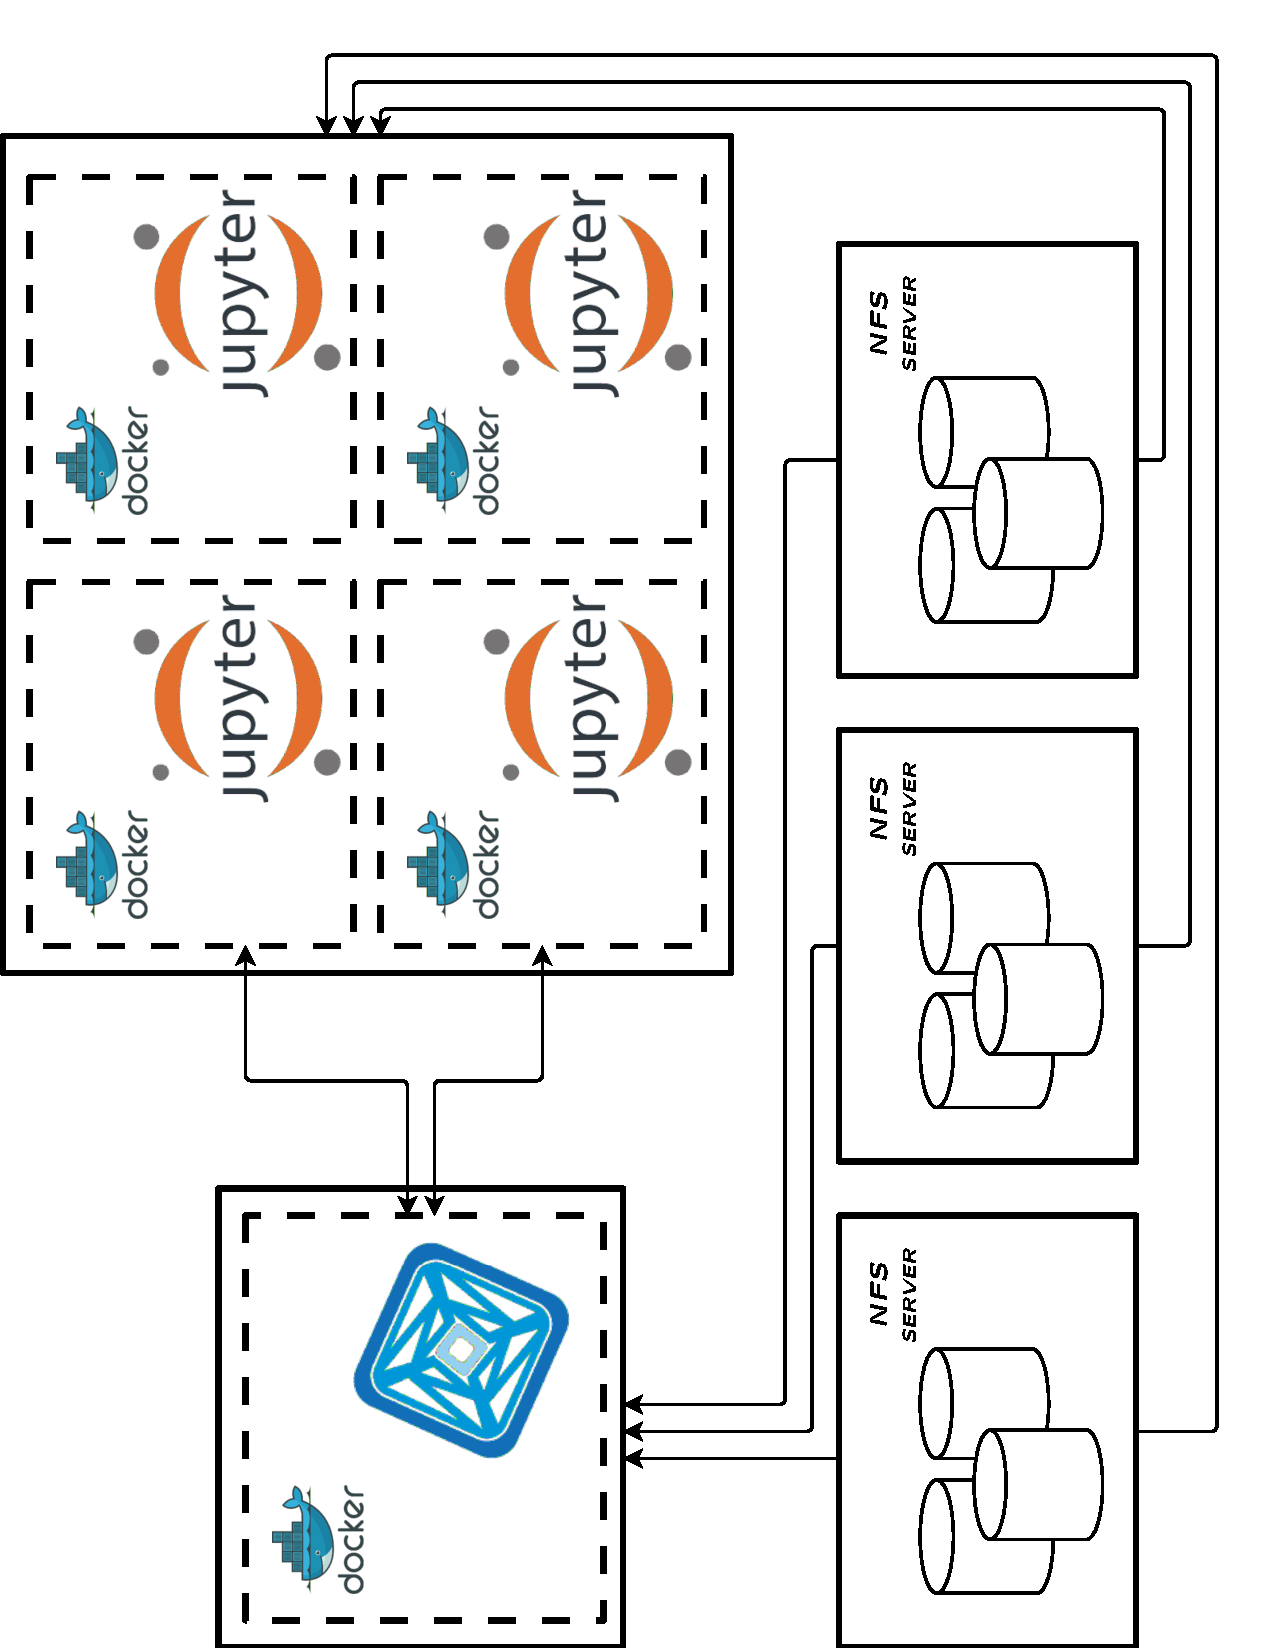
\includegraphics[angle=270, width=5.0in]{ythub_diagram}
\caption{Diagram showing the yt Hub structure}
\label{fig_sim}
\end{figure*}

\section{Concepts}

\subsection{Data management}
The physical location (filesystems) and form (POSIX files, databases) of data is
often dictated by the acquisition process, which is not necessarily relevant to
how the data is utilized during the analysis. It imposes the need of creating an
abstraction layer, that will allow to create a user friendly interface for
interacting with data. The yt Hub achieves this goal by exploiting Girder as a
data management framework. It allows to create dynamic data hierarchies that
transparently proxy data from \emph{Assetstores}, which represent raw data
storage backends. Datasets can be organized into \emph{Collections} that are the
top level objects, containing \emph{Folders} and \emph{Items}. \emph{Folders}
are a hierarchically nested organizational structure that consist of other
\emph{Folders} and \emph{Items}. \emph{Item} is the basic unit of data in the
system. \emph{Items} live beneath \emph{Folders} and contain zero or more
\emph{Files}, which represent raw data objects. Each organizational object, i.e.
\emph{Collection}, \emph{Folder} and \emph{Item} can be annotated with metadata
that is a simple key-value pair or JSON. Additionally Girder provides
basic authentication (\emph{Users}) and access control model for resource
management in form of \emph{Groups} of \emph{Users}.  
\par The capabilities of the Girder platform can be easily extended by
introduction of custom plugins that can modify both the server and web client
components. The yt Hub's specific extensions, including ability to spawn Jupyter
Notebooks with direct access to then data managed by Girder, is described in
detail in section~\ref{sec:ythub_plugin}.

\subsection{Data storage}
Data can be ingested into the Girder instance twofold: by \emph{uploading} or by
\emph{importing}. When uploaded, the files are stored on the NFS filesystem
underneath a specified directory. Files are named by their SHA-512 hash, which avoids
duplication of file content. If data is too big to be copied it is possible to
register location and size of the files within Girder via 'import' function. In
this case imported \emph{Items} are treated as integral part of Girder's data
collection. However, operations such as delete, move do not touch the actual
data and only work on model representation.

The yt Hub is capable of holding over 60TB of data utilizing OpenStack's block
storage service -- Cinder. Total disk capacity is divided into several block
devices. Each of them is mounted to a thin VM and shared over local network
using NFS. 

Every filesystem that holds true binary representation of data is simultaneously
mounted via NFS on computing resources and server hosting Girder using
identically named mountpoints. In order to increase the security of data, NFS
resources on computing nodes are mounted read-only.

\subsubsection*{brief info about ytHub plugin for girder}~\\
The ytHub plugin is complemented by a configurable-http-proxy (CHP) and a volume
manager (VolMan) that are running on compute node.

The ytHub plugin extends Girder with a new model: \emph{Notebook}. It keeps the
basic information about docker container that is running Jupyter Notebook, who
and when started it, and which Girder folder is mounted within the container:
\begin{lstlisting}[language=json,firstnumber=1]
  {
    "_id": <notebook obj uuid>
    "_modelType": "notebook",
    "containerId": <Docker container id>,
    "containerPath": <proxy suffix>,
    "created": <creation time>,
    "folderId": <folder obj uuid>,
    "lastActivity": <last access time>,
    "mountPoint": <FUSE mountpoint on host> 
    "userId": <user obj uuid>,
  }
\end{lstlisting}

ytHub plugin takes over some responsibilities of JupyterHub.

adding notebook model, requires only \verb|ythub.tmpnb_url| which is the
volman/chp endpoint

Girder's db model: folder id, user id, url, creation time (not used)

\subsection{Compute node}
describe Jupyter, chp

\section{Implementation}
\subsection{detailed description of ythub plugin}~\label{sec:ythub_plugin}

\begin{itemize}
\item GET \verb!/notebook!

list notebooks running for a specific folder and/or user

\item GET \verb!/notebook/{id}!

get model for notebook identified by id

\item POST \verb!/notebook/{id}!

if exists returns model else POSTs folder id and user id to volman, creates new
model if success

\item DELETE \verb!/notebook/{id}!

delete notebook using its id if belongs to user or user is admin

\end{itemize}

\subsection{detailed description of volman}

Runs tinydb. requires access to Docker daemon. Creating (POST):
\begin{enumerate}
   \item get username using token authentication
   \item create Docker volume
   \item identify mountpoint path on host (store in db: path)
   \item download ipynb from 'Private' directory
   \item mount bind folders / items if possible (store in db: target of mount)
   \item download remaining files if $\le 1$~Gb (asynchronously)
   \item start container (store in db: container id and url)
   \item add proxy path
   \item return url
\end{enumerate}

Destroying (DELETE):
\begin{enumerate}
   \item get username using token authentication
   \item check db for (user, folder) pair to get container id
   \item shutdown container
   \item unmount binds
   \item upload ipynb back to Girder
   \item remove volume
   \item remove db entry
\end{enumerate}

Imposes limits on running containers (cpu / memory)

\section{Use case}
Galaxy goes here

\section{Conclusion}
The conclusion goes here.
% use section* for acknowledgment
\section*{Acknowledgment}
The authors would like to thank... 

% trigger a \newpage just before the given reference
% number - used to balance the columns on the last page
% adjust value as needed - may need to be readjusted if
% the document is modified later
%\IEEEtriggeratref{8}
% The "triggered" command can be changed if desired:
%\IEEEtriggercmd{\enlargethispage{-5in}}

\bibliographystyle{IEEEtran}
\bibliography{IEEEabrv,ythub}
\end{document}
   
% vim:tabstop=3:shiftwidth=3:expandtab:textwidth=80:filetype=plaintex
